In this section, we introduce the system architecture for implementing our
opportunistic evaluation framework for dataframe query optimization within Jupyter notebooks. 
At a high level, we create a custom Jupyter Kernel to intercept dataframe queries in order to defer, schedule, and optimize them transparently. The query execution engine uses an operator DAG representation for scheduling and optimizing queries and caching results, and is responsible for scheduling asynchronous query executions during \thinktime. When new interactions arrive, the execution of non-critical operators is preempted and partial results are cached to resume execution during the next \thinktime. A garbage collector periodically uncaches results corresponding to the DAG nodes to avoid memory bloat based on the likelihood of reuse.


\subsection{Kernel Instrumentation}
\begin{figure}
    \centering
    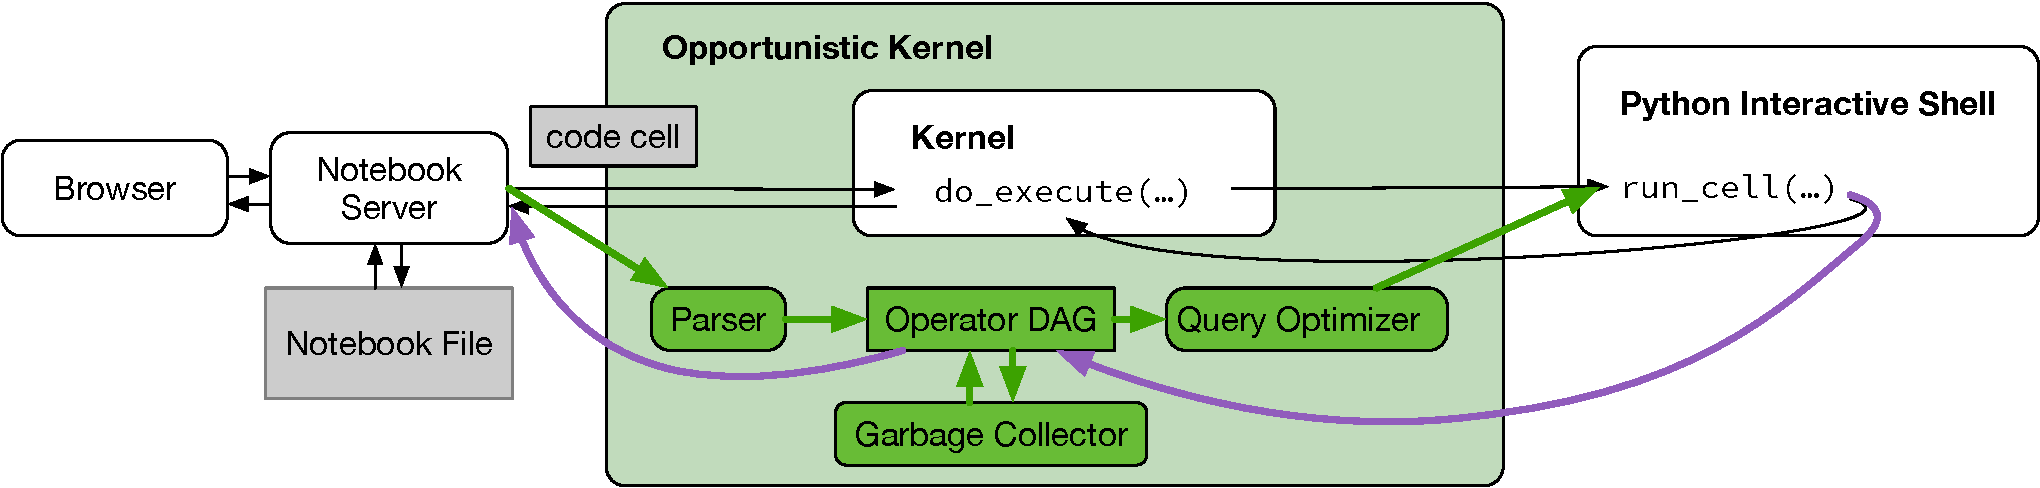
\includegraphics[width=0.7\textwidth]{submissions/interactivity/figures/kernel.pdf}
    \caption{Opportunistic Evaluation Kernel Architecture.}
    \label{fig:workflow}
    \vspace{-5mm}
\end{figure}

Figure~\ref{fig:workflow} illustrates the round-trip communication between the Jupyter front-end and the Python interactive shell. The black arrows indicate how communication is routed normally in Jupyter, whereas the green and purple arrows indicate how we augment the Jupyter Kernel to enable opportunistic evaluation. First, when the code is passed from the front-end to the kernel, it is intercepted by the custom kernel that we created by wrapping the standard Jupyter kernel. As shown in the green box, the code is passed to a parser that generates a custom intermediate representation, the operator DAG. The operator DAG is then passed to the query optimizer to create a physical plan for the query to be executed. This plan in then passed to the Python interactive shell for execution. When the shell returns the result after execution, the result is intercepted by the custom kernel to augment the operator DAG with runtime statistics as well as partial results to be used by future queries, and the query results are passed back to the notebook server, as indicated by the purple arrows.

\subsection{Intermediate Representation: Operator DAG}
\label{sec:dag}
\begin{figure}
    \centering
    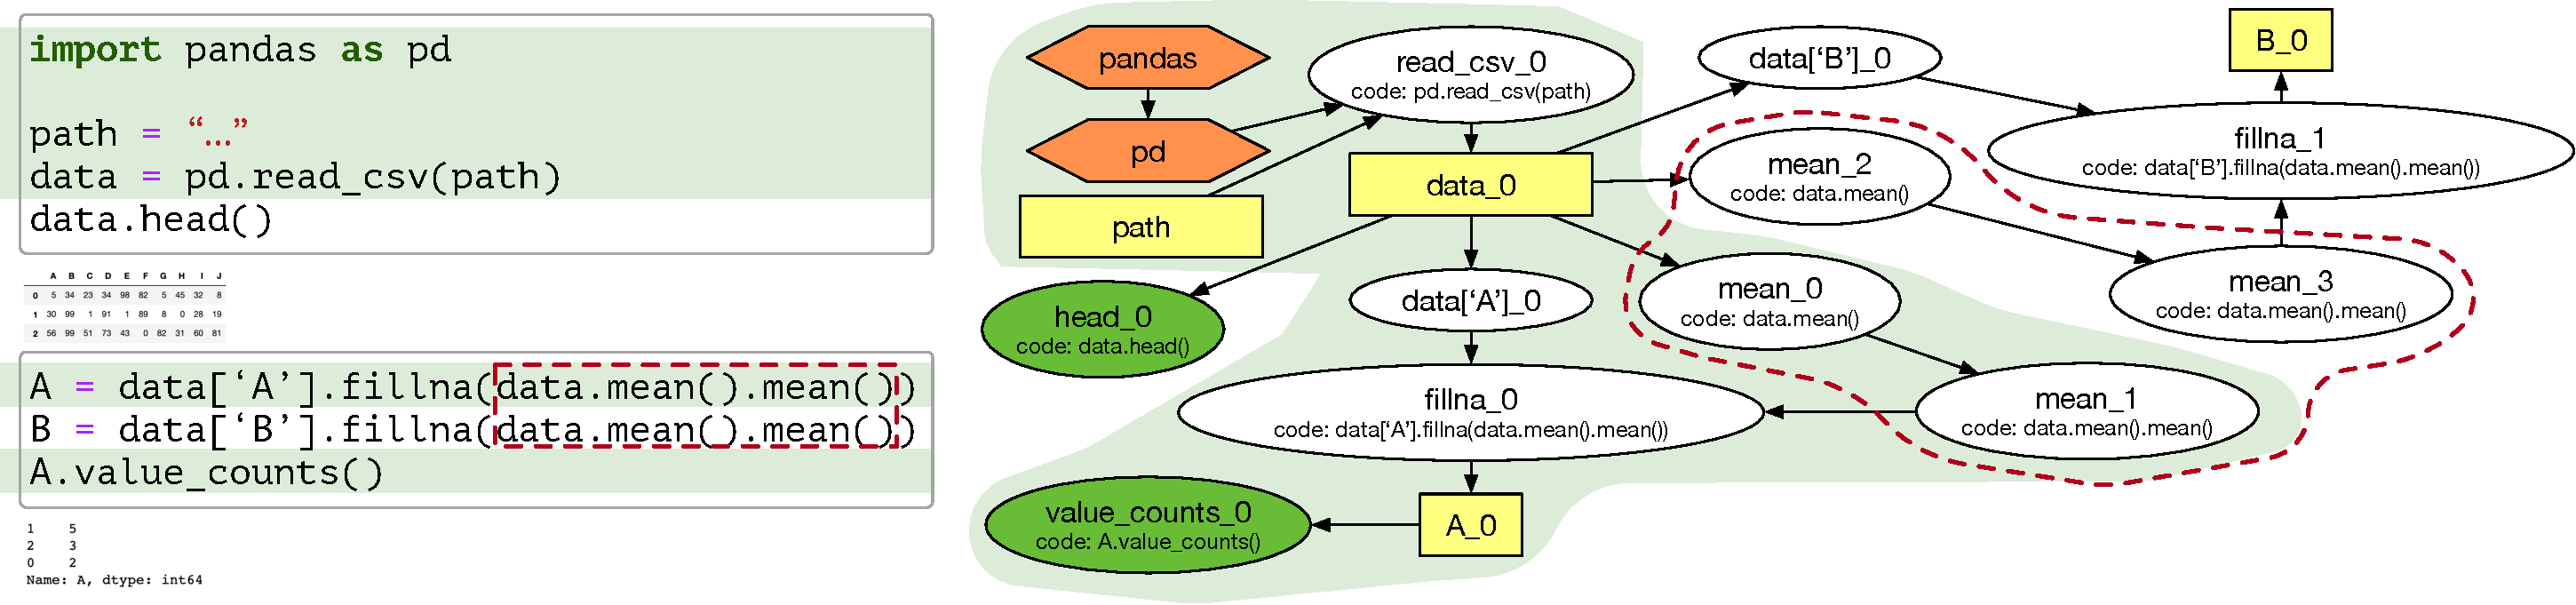
\includegraphics[width=0.8\textwidth]{submissions/interactivity/figures/dag.pdf}
    \caption{Example Code Snippet and Operator DAG.}
    \label{fig:op_dag}
    \vspace{-5mm}
\end{figure}

Figure~\ref{fig:op_dag} shows an example operator DAG constructed from the code snippet on the left. The orange hexagons are imports, yellow boxes are variables, ovals are operators, where green ovals are interactions. The operator DAG is automatically constructed by analyzing the abstract syntax tree of the code, in the parser component in Figure~\ref{fig:workflow}. We adopt the static single assignment form in our operator DAG node naming convention to avoid ambiguity of operator references, as the same operator can be invoked many times, either on the same or different dataframes. 
In the case that the operator DAG contains non-dataframe operators, we can simply project out the irrelevant operators by keeping only the nodes that are weakly connected to the \code{pandas} import node. 

To see how the operator DAG can be used for optimization, consider two simple use cases:

\topic{Critical path identification} To identify the critical path to the interaction \code{A.value\_counts()}, we can simply start at the corresponding node and traverse the DAG backwards to find all dependencies. Following this procedure, we would collect all nodes in the green region as the critical path to \code{A.value\_counts()} (corresponding statements are highlighted in green on the left), slicing out the operators associated with the statement \code{B = data[‘B’].fillna(data.mean().mean())}, which does not need to be computed for the interaction. 

\topic{Identifying repeated computation} Note that \code{data.mean().mean()} is a common subexpression in both \code{A} and \code{B}; recognizing this allows us to cache and reuse the result for \code{data.mean().mean()}, which is expensive since it requires visiting every element in the dataframe. We assume that operators are \textit{idempotent}, i.e., calling the same operators on the same inputs would always produce the same results. Thus, descendants with identical code would contain the same results. Based on this assumption, we eliminate common subexpressions by starting at the root nodes and traversing the graph breadth first, merging any descendants with identical code. We then proceed to the descendants of the descendants and carry out the same procedure until the leaf nodes are reached. Following this procedure, we would merge \code{mean\_0} with \code{mean\_2} and \code{mean\_1} with \code{mean\_3} in the red dotted region in Figure~\ref{fig:op_dag}.

We will discuss more optimizations in Section~\ref{sec:opt}.

\subsection{Operator Execution \& Garbage Collector}
When a notebook cell is executed, the opportunistic kernel first parses the code in the cell to add operators to the operator DAG described above. The DAG is then passed to the query optimizer, which will either immediately kick off the execution of interaction critical paths, if they are present in the DAG, or consider all the non-critical operators to determine what to execute next. We discuss optimizations for non-critical operators in Section~\ref{sec:non-critical}.

After the last interaction is executed and the results are returned, the query optimizer will continue executing operators asynchronously until the entire DAG is executed.
In the event that an interaction arrives while a non-critical operator is executing, we preempt the execution of the non-critical operator to avoid delaying the execution of the interaction critical path. We discuss optimizations for supporting effective preemption in Section~\ref{sec:critical}.

While the kernel executes operators, a garbage collector (GC) is working in the background to uncache results in the operator DAG to control memory consumption. A GC event is triggered when memory consumption is above 80\% of the maximum memory allocated to the kernel, at which point the GC inspects the operator DAG to uncache the set of operator results that are the least likely to speed up future queries. We discuss cache management in Section~\ref{sec:non-critical}.



